% -*- TeX -*-
\documentclass[aspectratio=169]{beamer}
\usepackage[none]{hyphenat}
\usepackage{minted}
\usepackage{tikz}

\usepackage{mathtools} % equations
\usepackage{booktabs} % tables

\title{PyLith v5.0 Tutorial}
\subtitle{Looking towards PyLith v6.0}
\author{Brad Aagaard\\
  Matthew Knepley \\
  Charles Williams}
\institute{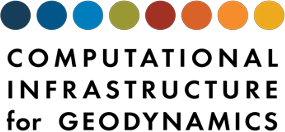
\includegraphics[scale=1.5]{../../logos/cig_logo_dots}%
  \hspace{4em}%
\raisebox{1em}{\includegraphics[scale=1.0]{../../logos/cig_short_pylith}}}
\date{June 9, 2026}


% TODO: Update development plan to move arrows on left

% ---------------------------------------------------- CUSTOMIZATION
\usetheme{CIG}
\input{../style}

% --------------------------------------------------------- DOCUMENT
\begin{document}

% ------------------------------------------------------------ SLIDE
\maketitle
\logo{\includegraphics[height=4.5ex]{../../logos/cig_short_pylith}}


% ========================================================== SECTION
\section{Ongoing development}

% ------------------------------------------------------------ SLIDE
\begin{frame}
  \frametitle{Development plan}
  \summary{}

    \only<1>{\includefigure[height=7.0cm]{figs/development-0}}
    \only<2>{\includefigure[height=7.0cm]{figs/development-1}}

\end{frame}


% ------------------------------------------------------------ SLIDE
\begin{frame}
  \frametitle{PyLith v5 release series}
  \summary{Finish reimplementation of PyLith v2 features}

  \begin{description}
    \item[v5.1] Reorganize finite-element kernels and do minor code clean up
    \item[v5.2] Dynamic prescribed slip, Drucker-Prager elastoplastic bulk rheology
    \item[v5.3] Quasistatic spontaneous rupture (friction)
  \end{description}
  
\end{frame}


% ------------------------------------------------------------ SLIDE
\begin{frame}
  \frametitle{PyLith v6}
  \summary{Major rewrite of user-facing code (Python/Pyre)}

  \begin{itemize}
  \item Update to current Pyre framework
  \item Address long-standing layout issues
  \item Add distribution via conda-forge
  \end{itemize}
  
\end{frame}


% ------------------------------------------------------------ SLIDE
\begin{frame}
  \frametitle{Update to current Pyre framework}
  \summary{}

  \begin{itemize}
    \hitem{Michael Aivazis has continued to develop Pyre, but we still use the "CIG" version from 2005}
    \begin{itemize}
      \item Requires a rewrite of PyLith's Python interface
      \item A few features needed by PyLith are missing from the current Pyre
    \end{itemize}
    \hitem{Redesign PyLith user interface from a user perspective}
    \begin{itemize}
      \item Design interface first and then rewrite underlying code to match
      \item Start with only Python code to facilitate iterative design
    \end{itemize}
    \hitem{Benefits}
    \begin{itemize}
      \item More intuitive specification of parameters (syntax and structure)
      \item Simpler implementation of components (easier to maintain and extend)
      \item Opportunity to address some long-standing user interface issues
      \item Facilitates coupling of components (useful in earthquake cycle modeling)
    \end{itemize}
  \end{itemize}
  
\end{frame}


% ------------------------------------------------------------ SLIDE
\begin{frame}
  \frametitle{Advantages of current Pyre framework}
  \summary{Maintained by original developer, Michael Aivazis}

  \begin{itemize}
  \item Improved journal support
  \item Simpler implementation of "components" in Python
  \item Improved application startup with support for subcommands
  \item Integration with SLURM scheduler for clusters
  \item Building blocks for a GUI
  \item Support for local, remote, and cloud filesystems
\end{itemize}

\end{frame}


% ------------------------------------------------------------ SLIDE
\begin{frame}
  \frametitle{PyLith redesign targets}
  \summary{Address long-standing user interface issues and prepare for the future}

  \begin{itemize}
  \item Reorganize directory structure into logical units matching user interface
  \item Restructure governing equations and materials (simplify user specification)
  \item Reformulate viscoelastic rheologies in terms of strain rate
  \item Examples as notebooks
  \item Set foundation for future features
    \begin{itemize}
    \item 4D specification of boundary conditions
    \item Earthquake cycle modeling
    \item Interaction (injection, output) with other codes
    \end{itemize}
  \end{itemize}

\end{frame}


% ------------------------------------------------------------ SLIDE
\begin{frame}[t,fragile]
  \frametitle{Switch from Config files to YAML files}
  \summary{Slightly simplified excerpts of PyLith parameter files}

  \begin{minipage}[t]{0.45\textwidth}
    {\scriptsize PyLith v5}
      \begin{cfgcode}
        [pylithapp.problem.mesh_initializer]
        read_mesh.filename = mesh_quad.msh

        [pylithapp.problem]
        bc = [bc_xneg, bc_xpos]
        bc.bc_xpos = pylith.bc.NeumannTimeDependent

        materials = [crust]

        [pylithapp.problem.materials.crust]
        label_name = material-id
        label_value = 1

        auxiliary_db = spatialdata.SimpleDB
        auxiliary_db.filename = mat_crust.spatialdb

        # etc.
      \end{cfgcode}
  \end{minipage}
  \hfill
  \begin{minipage}[t]{0.45\textwidth}
    {\scriptsize PyLith v6 (design in progress)}
      \begin{yamlcode}
        pylith.app.problem.mesh_initializer:
          read_mesh.filename: mesh_quad.msh

        pylith.app.problem.governing_eqn:
          boundary_conditions:
            - dirichlet#bc_xneg
            - neumann#bc_xpos
          materials:
            - isotropic_linear#crust

        crust:
          label_name: material-id
          label_value: 1
          auxiliary_db: spatialdata.SimpleDB#db_crust:
        db_crust:
          filename: mat_crust.spatialdb

        # etc.
      \end{yamlcode}
  \end{minipage}
  
\end{frame}


% ------------------------------------------------------------ SLIDE
\begin{frame}
  \frametitle{Examples as notebooks}
  \summary{}

  \begin{itemize}
  \hitem{Integrate explanation, parameter specification, and visualization into a notebook}
    \begin{itemize}
      \item Examples are self-contained, reducing duplication
      \item Integrated visualization
      \end{itemize}
  \hitem{Candidate implementation: marimo notebooks (next-generation Python notebook)}
    \begin{itemize}
      \item Change a cell, and dependent cells refresh
      \item Interactive widgets
      \item Stored as Python
      \item No hidden state
      \item Run as a Python script or interactive notebook
    \end{itemize}
  \end{itemize}
\end{frame}
 

% ------------------------------------------------------------ SLIDE
\begin{frame}
  \frametitle{PyLith Graphical User Interface}
  \summary{}

  \begin{itemize}
    \hitem{PyLith Parameter Viewer}
    \begin{itemize}
      \item View parameters that were saved at beginning of simulation.
    \end{itemize}
    \hitem{New GUI}
    \begin{itemize}
      \item Configuration of parameter files
      \item Monitor a running simulation \\
      \noindent\vdots
    \end{itemize}
  \end{itemize}

\end{frame}


% ------------------------------------------------------------ SLIDE
\begin{frame}
  \frametitle{PyLith Graphical User Interface}
  \summary{Development plan}

  \begin{enumerate}
    \item Graphical view of component hierarchy from parameter files
    \item Monitoring of running simulation (e.g., activate/deactivate journals)
    \item Synchronized editing of parameter files using graphical view or text \\
    \noindent\vdots
    \item Steer running simulation (e.g., journals on/off)
    \noindent\vdots
    \item Visualization of solution and state variables from running simulation \\
  \end{enumerate}

\end{frame}


% ------------------------------------------------------------ SLIDE
\begin{frame}[t]
  \frametitle{Bayesian Inversion = PyLith + AlTar}
  \summary{Background}

  \begin{itemize}
    \hitem{Sarah Minson's CATMIP code}
      \begin{itemize}
      \item Not yet open-source
      \item Portability and usability issues
      \item Used in 2023 PyLith hackathon but PyLith$\rightarrow$CATMIP integration needs work
      \end{itemize}
    \hitem{Open-source AlTar (Albert Tarantola)}
      \begin{itemize}
      \item Michael Aivazis worked with Sarah to implement CATMIP algorithm in Python/C++ using his Pyre
      \item Lijun Zhu (Caltech) has continued developing AlTar
      \item We have started working with Lijun Zhu and Michael to make AlTar more accessible
        \begin{itemize}
        \item Objective: "CIGize" AlTar
        \item Modular, flexible interface between PyLith (Green's functions) and AlTar
        \item Facilitate AlTar becoming a community code
        \end{itemize}
      \end{itemize}
  \end{itemize}

\end{frame}


% ------------------------------------------------------------ SLIDE
\begin{frame}
  \frametitle{Ongoing PyLith development}

  \begin{itemize}
  \item Ambitious development plan
    \begin{itemize}
    \item Human resources are limited (other obligations)
    \item Leverage AI coding agents to accelerate process (Friday discussion)
    \end{itemize}
  \item Collaborations and community engagement are important!
    \begin{itemize}
    \item Help refine priorities
    \item Contribute via hackathons, reporting errors, improving documentation
    \item Give appropriate attribution
    \end{itemize}
  \end{itemize}

\end{frame}


% ======================================================================
\end{document}


% End of file
